\documentclass[english,final,hyperref={pdfpagelabels=false}]{beamer}
\usepackage[utf8]{inputenc}
\usepackage{graphicx}
\usepackage{booktabs}
\usepackage{array}
\usepackage{wrapfig}
\usepackage{xcolor}
\usepackage[orientation=portrait,size=a0,scale=1.25]{beamerposter}
\mode<presentation>{
    \usetheme{_lulav_poster}
}

\begin{document}
\title[]{Hornbill C-UAS Series}
\author[]{Lulav - Micro Defense Systems}
% \date[]{August 2025}
\setbeamercolor{background canvas}{bg=taskyblue}
\begin{frame}{ }
% --- Top images ---
\begin{center}
% 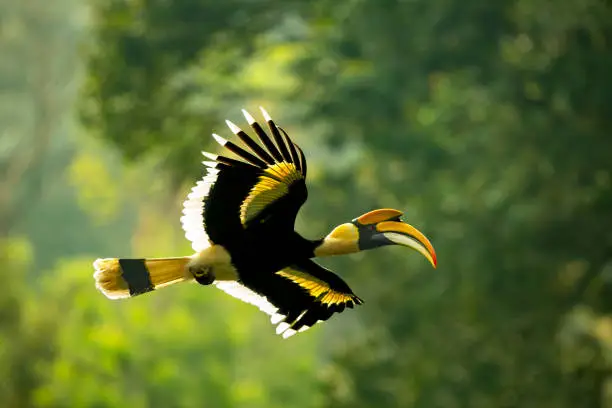
\includegraphics[width=0.45\textwidth]{hornbill_image.png}
% \hspace{2em}
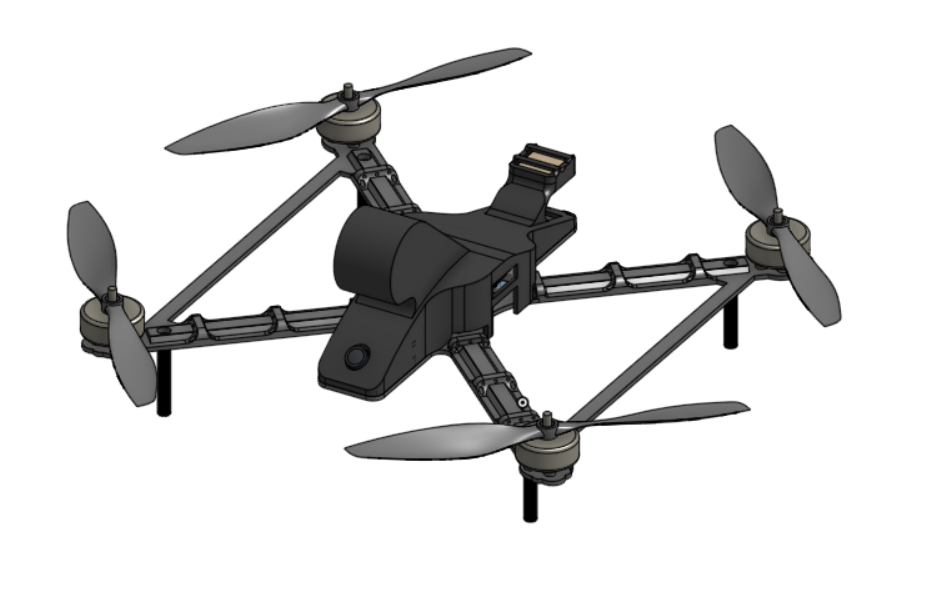
\includegraphics[width=0.45\textwidth]{lulav_hornbill.png}
\end{center}
\vfill
% --- Mission ---
\begin{block}{\Large Mission}
\large The \textbf{Lulav Hornbill} is a kinetic interceptor inspired by the agility of the hornbill bird. 
It delivers rapid, autonomous interception of hostile Class 1--2 UAS, day or night, with seamless integration to modern C2 systems and direct sensor ingest (Radar/EO/IR).
\end{block}
% --- Columns for content ---
\begin{columns}[t]
\column{0.32\textwidth}
\begin{block}{\Large Performance}
\begin{center}
\begin{tabular}{>{\bfseries}m{0.35\linewidth} m{0.5\linewidth}}
Range Band & Speed Envelope \\\midrule
2--5 km  & 40--70 m/s \\
5--10 km & 30--60 m/s \\
10--20 km & 25--50 m/s \\
\end{tabular}
\end{center}
\vspace{1ex}
\textbf{Day/Night Interception}: Optimized for visual and RF-degraded conditions.

\textbf{Effective Classes}: 1--2 UAS.
\end{block}

\column{0.32\textwidth}
\begin{block}{\Large Integration}
\begin{itemize}
    \item \textbf{C2}: Standards-based integration to tactical C2 networks.
    \item \textbf{Direct Sensors}: Radar and EO/IR direct ingest for low-latency tasking.
    \item \textbf{Autonomy}: Full mission autonomy from launch to intercept, with operator-in-the-loop options.
\end{itemize}
\end{block}

\column{0.32\textwidth}
\begin{block}{\Large Key Features}
\begin{itemize}
    \item \textbf{Kinetic Intercept}: Hard-kill solution with minimal collateral effects.
    \item \textbf{Agile Guidance}: High authority attitude control and pursuit logic.
    \item \textbf{Modular Airframe}: Field-swappable battery/payload modules.
    \item \textbf{Ruggedized Ops}: Rapid setup; mobile launch compatible.
\end{itemize}
\end{block}

\end{columns}

\vfill

\begin{block}{\Large Summary}
\large \textbf{Hornbill} combines speed, precision, and autonomy for decisive C-UAS defense across short to medium ranges, providing a robust, cost-effective hard-kill option.
\end{block}

% \begin{block}{\Large Contact}
% \textbf{Lulav Space Ltd.}\\
% Haifa, Israel\\
% \texttt{info@lulav.space} \quad \texttt{www.lulav.space}
% \end{block}

\end{frame}
\end{document}
